% !Mode:: "TeX:UTF-8"
\documentclass{xcumcmart}
\usepackage{setspace}
\usepackage{enumerate}
\usepackage{graphics}
\usepackage{tabu}

% \title{text}这里是显示在第三页的文章标题
\title{关于科学艺术的综述}
% \author{何长鸿 2016141482154}

\linespread{1.5} %行距
\CTEXsetup[format={\Large\bfseries}]{section} %章节标题左对齐
\setlength{\parskip}{1.4em} %1.4倍段落距离

\begin{document}

\renewcommand\arraystretch{2}
\maketitle
\begin{abstract}
\par 印象主义是19世纪的一个艺术运动,最初是19世纪60年代巴黎艺术家的松散联盟,他们公开展示自己的艺术。这场运动的名字来源于克劳德莫奈的作品《印象日出》的标题,它激起了评论家路易斯勒罗伊在讽刺评论中提出了这个词。印象派绘画的特点包括可见的笔触,以及强调光的变化特性(通常强调时间流逝的影响),普通的题材。本文将结合具体作品对印象派艺术绘画历史以及其特点展开论述,并将介绍一些印象派的画作。
\newline
\par\textbf{关键词:印象派 发展历史 风格特点}    
\end{abstract}
\section{印象派绘画的起源}
\par 在画坛众多的派别中,西洋油画中的印象派一直为西方人所 推崇。印象派起源于法国,尽管大多数说法认为此流派的创始人是莫奈,但真正的起源,是主张“为艺术而艺术”的法国绘画大师——马奈。虽然他从未真正参加印象派的展览,但他深具革新精神的艺术创作态度,却深深影响了莫奈,塞尚、凡·高等新兴画家,进而将绘画带入现代主义的道路上。受到日本浮世绘及西班牙画风的影响,马奈大胆采用鲜明色彩,舍弃传统绘画的中间色彩,将绘画从追求三元次立体空间的传统束缚中解放出来,朝二元次的平面创作迈出革命性的一大步。主要表现在《草地上的午餐》(图\ref{cdsdwc.jpeg})和《奥林匹亚》(图\ref{fig:alpy.jpeg})画中的裸女,以同一种肤色描绘人体就可以看出。
\begin{figure}[htbp]
    \centering
    \begin{minipage}[htbp]{0.48\linewidth}
        \centering
        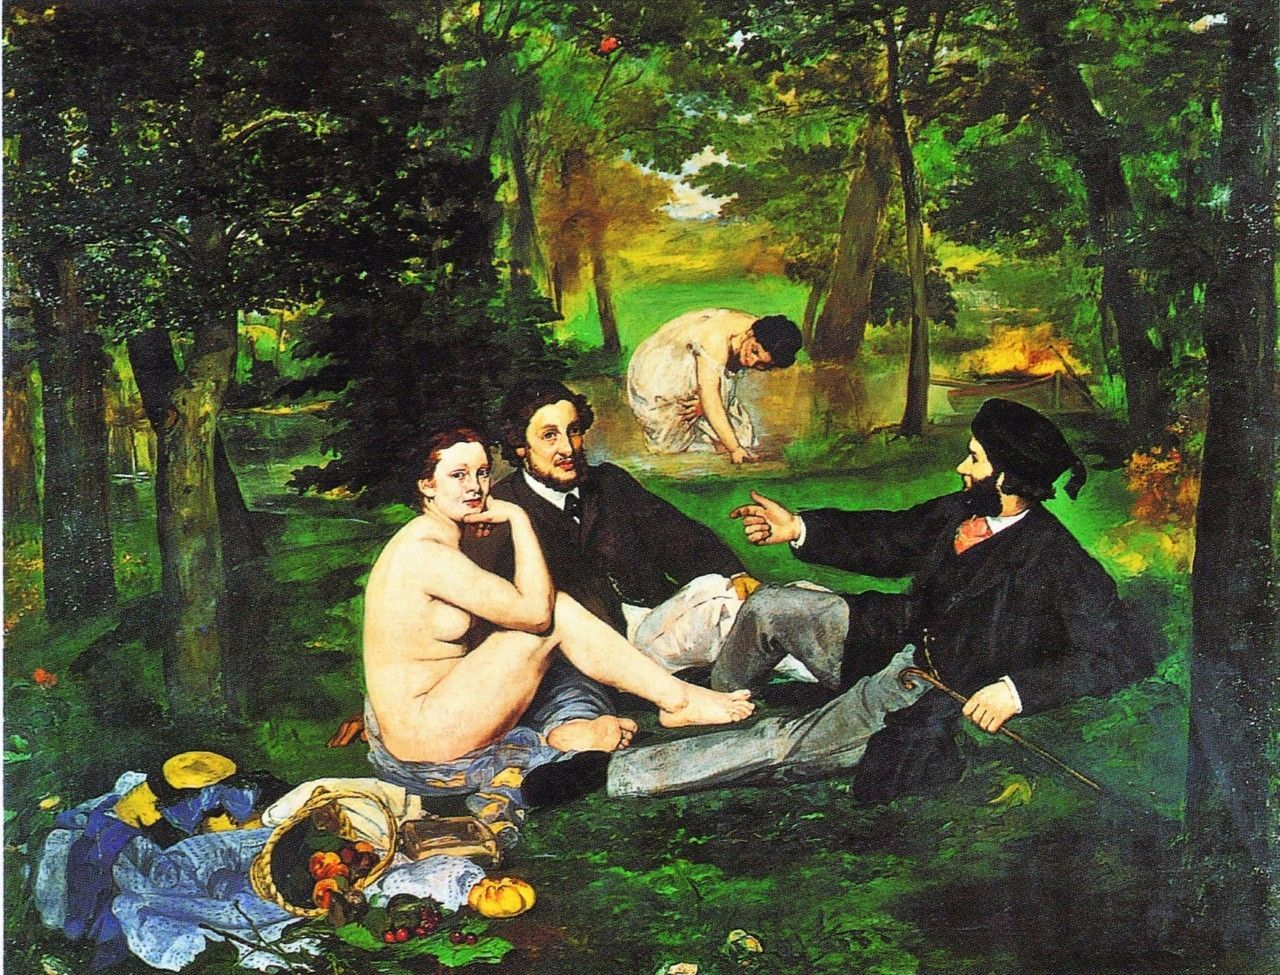
\includegraphics[width=1\textwidth,height=6cm]{fig/cdsdwc.jpeg}
        \caption{草地上的午餐\label{fig:cdsdwc.jpeg}}
    \end{minipage}
    \hfill
    \begin{minipage}[htbp]{0.48\linewidth}
        \centering
        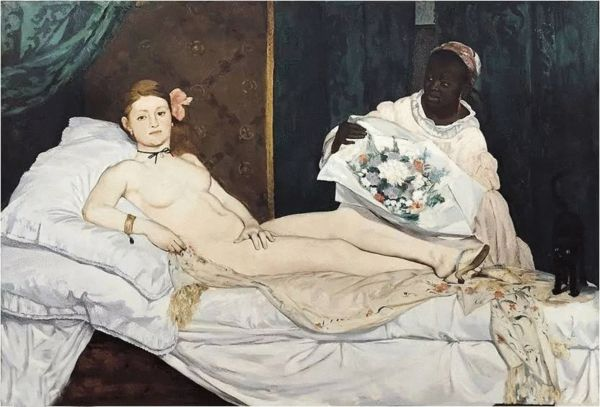
\includegraphics[width=1\textwidth,height=6cm]{fig/alpy.jpg}
        \caption{奥林匹亚\label{fig:alpy.jpeg}}
    \end{minipage}
    \end{figure}
\par 此外,马奈亦以自然主义式的想像来处理创作的题材与构图,并未刻意美化,取而代之的是清晰、冷静、光线均匀分布的景致,表现出和谐、清楚而简约的风格。马奈在绘画生涯的大胆创新,影响深远,在美术史上可谓占有举足轻重的地位。
\par 再接下来该出场的就是莫奈,莫奈对这一艺术环境的形成和他描绘现实的新手法,比其他任何人贡献都多。这一点是无庸置疑的,印象派的创始人虽说是马奈,但真正使其发扬光大的却是莫奈,因为他对光影之于风景的变化的描绘,已到走火入魔的境地。
\par 他对光色的专注远远超越物体的形象,使得物体在画布上的表现消失在光色之中。他让世人重新体悟到光与自然的结构。所以这一视野的嬗变,以往甚至难以想象,它所散发出的光线、色彩、运动和充沛的活力,取代了以往绘画中僵死的构图和不敢有丝毫创新的传统主义。
\par 印象派作为油画重要派别,它的名称起源于法国画家莫奈的 一幅画。1874年,在巴黎摄影师纳达尔的工作室里,两位艺术家 看到莫奈的一幅名为“日出印象”的画,便把这种突破传统画法的 画称为“印象”,从这以后“印象派”就被用来称呼当时一批突破传统画法的年轻画家。
\section{印象派绘画的特点}
\par 印象主义派以色彩为中心,创立了不同于以往任何图式的视觉语言,拉开了西方现代美术的序幕,印象主义的产生,与几个客观条件息息相关,首先,不论从技术还是效果上,安格尔式新古典主义绘画都可谓以穷极写实注意,倘若再沿着着条路走下去,除了重复,画家们不可能走的更远,19世纪物理科学的进步,是导致印象主义产生的直接条件,当时色彩学被一次科学的对应与光学,从而揭示了物理学本质,人们认识到,色彩并非物体的属性,而是光的折射在视网膜上所造成的知觉反映,光线变化了,色彩也随之变化\cite{2},这些人认识被反映在法国人谢弗勒尔的《色彩对比论》和美国人O·N·鲁特的《现代色彩学》西部代表性著作中。而他们所阐述的色彩对比与视觉调和的原理,正是印象派画家所实行的东西。
\par 印象派语言的出现,是以观念的改变为前提,这种观念与库尔贝式现实注意一脉相承,在放弃追求普遍性和类型化的古典主义艺术理想之后,印象派破除事物具有恒常性的看法,将艺术的触觉深入到大千世界生生不息的变化之中,以表现瞬间真实为己任。总结印象派绘画大概有以下三个特点:
\subsection{表现瞬间真实}
\par 印象派语言的出现,是以观念的改变为前提,这种观念与库尔贝式现实注意一脉相承,在放弃追求普遍性和类型化的古典主义艺术理想之后,印象派破除事物具有恒常性的看法,将艺术的触觉深入到大千世界生生不息的变化之中,以表现瞬间真实为己任。
\subsection{以光和色彩为表现媒介}
\par 印象主义者抛弃了支配欧洲绘画数百年的固有观念,将色彩直根与光学研究之新成果所提供的信念中,当下即得地捕捉有某一瞬间的光线作用所造成的色彩印象,致力于表现光源色和条件色,从而表现出大自然在一刻也不停的变化之中所呈现的美,正如他们自己所说,印象主义旨在使艺术回到一种严格认真的,精确的对于大自然的观察,使我们自己热忱的在运动之中也在光的瞬间描绘形状。“

\par 文艺复兴以来的欧洲绘画发展了一种以素描为中心的图式,这种图式建立在物体坚实不变的信念基础上,所瞄准的是结构而不是光线,所看到的是明暗而不是色彩,印象派则将色彩置于画面的中心地位,又使一切色彩皆从光源色出发,力图表现出太阳的,真正的光,他们完全打破了户外搜集素材,户内整理加工的风景画创作模式,多数时候在户外光线下直接完成作品,同时,他们强调,既然万物都受太阳照射,那么,任何一个对象的色彩都不可能是独立的而必然以周围物体的反射光为条件,因此,也特别注意反映条件色,正是光源色与条件色,将印象派的画圈变成了一个统一与色彩中的整体。
\subsection{突出绘画的视觉性}
\par 印象派追求的“画其所见”,以描绘艺术家所看到的视觉表象为宗旨,而不强调表现事物背后的意义。他们以色彩作为光的回声,建立色彩的和谐,谱写视觉的音乐,使绘画回到了视觉艺术的位置上,不过,对光线与色彩的敏感加深了印象派画家对大千世界运动的本质的感悟。如果说,印象派绘画有什么内容意义的话,那就是它们以可见的形式结构了生长与衰灭不断交替进行的节奏,让我们直接看到了生命与自然运动的本质。\cite{1}

\begin{thebibliography}{1}
    \bibitem{1} xgopf4,印象派绘画在现代艺术发展中的地位和作用,https://blog.csdn.net/xgopf4/article/details/3560999,2008.
    \bibitem{2} Ogden Nicholas Rood,色彩现代学.
\end{thebibliography}
\end{document}
